\documentclass[
	a4paper,
	oneside,
	DIV = 12,
	fontsize = 13pt,
	headings = normal,
]{scrartcl}

%%% Page geometry and precise margins
\usepackage[
	pass,
	left   = 20mm,
	top    = 15mm,
	right  = 10mm,
	bottom = 15mm,
]{geometry}
%%%

%%% Length calculations
\usepackage{calc}
%%%

%%% Support for color
\usepackage{xcolor}
\definecolor{lightblue}{HTML}{03A9F4}
\definecolor{red}{HTML}{F44336}
%%%

%%% Including graphics
\usepackage{graphicx}
%%%

%%% Font selection
\usepackage{fontspec}

\setromanfont{STIX Two Text}[
	SmallCapsFeatures = {LetterSpace = 5},
]

\setsansfont{IBM Plex Sans}[
	Scale = MatchUppercase,
]

\setmonofont{IBM Plex Mono}[
	Scale = MatchUppercase,
]
%%%

%%% Math typesetting
\usepackage{amsmath}

\usepackage{unicode-math}
\setmathfont{STIX Two Math}
%%%

%%% List settings
\usepackage{enumitem}
\setlist[enumerate]{
	label*      = {\arabic*.},
	leftmargin  = *,
	labelindent = \parindent,
	topsep      = 1\baselineskip,
	parsep      = 0\baselineskip,
	itemsep     = 1\baselineskip,
}

\setlist[itemize]{
	label       = {—},
	leftmargin  = *,
	labelindent = \parindent,
	topsep      = 1\baselineskip,
	parsep      = 0\baselineskip,
	itemsep     = 1\baselineskip,
}

\setlist[description]{
	font        = {\rmfamily\upshape\bfseries},
	topsep      = 1\baselineskip,
	parsep      = 0\baselineskip,
	itemsep     = 0\baselineskip,
}

%%%

%%% Structural elements typesetting
\setkomafont{pagenumber}{\rmfamily}
\setkomafont{disposition}{\rmfamily\bfseries}

% Sectioning
\RedeclareSectionCommand[
	beforeskip = -1\baselineskip,
	afterskip  = 1\baselineskip,
	font       = {\normalsize\bfseries\scshape},
]{section}

\RedeclareSectionCommand[
	beforeskip = -1\baselineskip,
	afterskip  = 1\baselineskip,
	font       = {\normalsize\bfseries},
]{subsection}

\RedeclareSectionCommand[
	beforeskip = -1\baselineskip,
	afterskip  = 1\baselineskip,
	font       = {\normalsize\bfseries},
]{subsubsection}
%%%

%%% Typographic enhancements
\usepackage{microtype}
%%%

%%% Language-specific settings
\usepackage{polyglossia}
\setmainlanguage{ukrainian}
\setotherlanguages{english, russian}
%%%

%%% Captions
\usepackage{caption}
\usepackage{subcaption}

%\DeclareCaptionLabelFormat{closing}{#2)}
%\captionsetup[subtable]{labelformat = closing}

%\captionsetup[subfigure]{labelformat = closing}

\captionsetup[table]{
	aboveskip = 0\baselineskip,
	belowskip = 1\baselineskip,
}

\captionsetup[figure]{
	aboveskip = 1\baselineskip,
	belowskip = 0\baselineskip,
}

\captionsetup[subfigure]{
	aboveskip = 0.25\baselineskip,
	belowskip = 0\baselineskip,
}

\captionsetup[subfigure]{
	labelformat = simple,
	labelformat = brace,
}
%%%

%%% Table typesetting
\usepackage{booktabs}
\usepackage{longtable}

\usepackage{multirow}

\usepackage{array}
\newcolumntype{v}[1]{>{\raggedright\arraybackslash\hspace{0pt}}p{#1}}
\newcolumntype{b}[1]{>{\centering\arraybackslash\hspace{0pt}}p{#1}}
\newcolumntype{n}[1]{>{\raggedleft\arraybackslash\hspace{0pt}}p{#1}}
%%%

%%% Dingbats
\usepackage{pifont}
%%%

%%% TikZ
\usepackage{tikz}
%%%

%%% Links and hyperreferences
\usepackage{hyperref}
\hypersetup{
	bookmarksnumbered = true,
	colorlinks      = false,
	linkbordercolor = red,
	urlbordercolor  = lightblue,
	pdfborderstyle  = {/S/U/W 1.5},
}
%%%

%%% Length adjustments
% Set baselineskip to ~15pt, default is 14.5pt
% \linespread{1.034483}
% \linespread{1.068966} % ~15.5pt
\setlength{\emergencystretch}{1em}
\setlength{\parindent}{1.5em}
\newlength{\gridunitwidth}
\setlength{\gridunitwidth}{\textwidth / 12}
\setlength{\floatsep}{1\baselineskip}
\setlength{\intextsep}{1\baselineskip}
\setlength{\textfloatsep}{1\baselineskip}
%%%

%%% Custom commands
\newcommand{\allcaps}[1]{{\addfontfeatures{LetterSpace = 5}#1}}
\newcommand{\progname}[1]{\texttt{#1}}

\newcommand{\CheckMark}{\ding{51}}
\newcommand{\Mytextrightarrow}{$\rightarrow$\hspace{0.25em}}
%%%

%%% Make typography adhere to made-up standards
\PolyglossiaSetup{ukrainian}{indentfirst = true}

% Sectioning
\RedeclareSectionCommand[
	beforeskip = -0sp,
	afterskip  = 1sp,
	indent     = 12.5mm,
	font       = {\normalsize\bfseries},
]{section}

\RedeclareSectionCommand[
	beforeskip = -0sp,
	afterskip  = 1sp,
	indent     = 12.5mm,
	font       = {\normalsize\bfseries},
]{subsection}

\RedeclareSectionCommand[
	beforeskip = -0sp,
	afterskip  = 1sp,
	indent     = 12.5mm,
	font       = {\normalsize\bfseries},
]{subsubsection}

\setlength{\parindent}{12.5mm}

\usepackage{leading}
\leading{21pt}

%%%

\begin{document}
	\newgeometry{
		left   = 20mm,
		top    = 15mm,
		right  = 10mm,
		bottom = 15mm,
		footskip = \baselineskip, % reduce footer vertical skip so page numbers are visible
	}
\setlength{\gridunitwidth}{\textwidth / 12}
	\begin{titlepage}
		\begin{center}
			Міністерство освіти і науки України\\
			Національний авіаційний університет\\
			Навчально-науковий інститут комп'ютерних інформаційних технологій\\
			Кафедра комп'ютеризованих систем управління

			\vspace{\fill}
				Лабораторна робота №4\\
				з~дисципліни «Діагностика та~експлуатація комп'ютера»\\
				на~тему «Резервне копіювання операційної системи»\\

			\vspace{\fill}

			\begin{flushright}
				Виконав:\\
				студент \allcaps{ННІКІТ}\\
				групи СП-325\\
				Клокун В.\,Д.\\
				Перевірив:\\
				Масловський Б.\,Г.
			\end{flushright}

			Київ 2018
		\end{center}
	\end{titlepage}

	\section{Ціль роботи}
		Ознайомлення з процесом резервного копіювання операційної системи.

	\section{Короткі теоретичні відомості}
		З моменту придбання персонального комп'ютера і до його запуску будь-якому користувачеві доводиться виконати ряд дій по попередньому налаштуванні. В першу чергу встановлюється операційна система, потім необхідні драйвери пристроїв і устаткування, після чого приходить черга програмного забезпечення. Нерідко, придбавши персональний комп'ютер або ноутбук, користувачі отримують вже готовий до роботи пристрій: ОС і драйвери встановлені тим, хто збирав комп'ютер, іноді навіть присутній мінімальний комплект офісного ПЗ. Не заважаючи на це, майже завжди потрібно виконати додаткові налаштування, такі як зміна зовнішнього вигляду ОС та встановлення додаткового ПЗ. Ці налаштування займають певний час. Цей час можна скоротити, якщо створити резервну копію ОС з усіма налаштуваннями.

		Завдання створення образу для повністю налаштованої операційної системи вже давно успішно вирішене розробниками програмного забезпечення. Продукти, за допомогою яких це робиться, існують в різних видах: є комерційні, є і безкоштовні. 

		Розглянемо процес виготовлення образу на прикладі \textenglish{Acronis True Image Home}. Перше, що треба зробити,~— створити диск, з якого можна завантажити комп'ютер. Він дозволить при фатальному збої (аж до виходу з ладу жорсткого диска) завантажитися з оптичного приводу, а потім з зовнішнього сховища відновити систему зі збереженого образу (в тому числі і на новий Hdd). Для цього необхідно в розділі «Інструменти і утиліти» вибрати пункт «Створення завантажувального носія». До речі, якщо ви вперше запустили \textenglish{Acronis True Image Home}, виконати цю процедуру вам буде запропоновано майстром. Образ диску, що Ви створили, можна зберегти у форматі \textenglish{ISO}, він невеликий за розміром~— близько 60 Мбайт, що дозволяє записати його навіть на флешку або маленький \textenglish{CD}. В процесі створення диска вам доведеться вибрати тільки пристрій для запису (або шлях для збереження образу \textenglish{ISO}). Після натискання кнопки «Приступити» у вас з’явиться або готовий \textenglish{CD}, або образ, який потрібно буде записати програмою для роботи з образами дисків на оптичний носій.

		Отже, завантажувальний диск готовий, можна приступити до процедури створення образу системного диска. Ідеальним випадком є створення образу саме з завантажувального диска: відсутній ризик втрати критично важливих даних через відкритих файлів і~т.\,д. Втім, те ж саме можна зробити і~з-під запущеної ОС: як показали експерименти, проблем з такий спосіб не виникає теж. 

		На вкладці «Стартова сторінка» вибираємо опцію-посилання «Диски» в рубриці «Резервне копіювання», вибираємо системний диск. На наступній вкладці вибираємо шлях для збереження образу. Важливо, щоб він ні в якому разі не перебував на системному диску; найкраще, якщо він розташований на зовнішньому носії та фізично іншому диску. Натискаємо кнопку «Приступити» та через час отримаємо образ системи. Для надійності цю операцію слід виконати один раз для нової, встановленої і налаштованої ОС, а потім кожні три місяці створювати архів поточного стану. Зрозуміло, перший з них необхідно зберегти в цілості і без змін, а оновлюваний можна зберігати не більше двох: поточний і попередній. 

		Якщо необхідно відновити образ з резервної копії, процедура виконується аналогічним чином: завантажуємося з завантажувального компакт-диска, вибираємо опцію «Відновити з резервної копії», вказуємо місце розташування останнього архіву (або самого першого, в залежності від ситуації), очікуємо 15-20 хвилин і отримуємо повністю працездатну систему. Можливо відновити копію і з операційної системи, правда, такий режим може використовуватися тільки для відновлення деяких файлів або папок, не зайнятих системними операціями або службами. Таким чином можна повернути в робочий стан випадково видалені або пошкоджені вірусами додатки. 

		Для цього треба вибрати вкладку «Відновлення» - «Відновлення дисків з резервної копії» і після вибору актуального образу в вікні «Виберіть метод відновлення» вказати, куди і які об'єкти розгортати. Необхідну інформацію можна помістити як в те ж саме місце, так і в окремий розділ: це може знадобитися для порівняння змінених файлів 

		\subsection*{Чому образ операційної системи варто резервувати}

		Незважаючи на розмір архівного файлу (а тільки в разі «нової ОС» він займе не менше 4{,}5~Гбайт), не треба економити місце для нього. Тому в ідеалі на зберігання слід помістити п'ять архівів: повністю встановлену та налаштовану ОС з драйверами; повністю підготовлену до роботи систему з встановленим ПО; щорічну копію робочої конфігурації і дві оновлювані щоквартальні копії, останню і попередню. 

		Такий режим зберігання гарантовано дозволить уникнути будь-яких проблем з можливим пошкодженням як ПО, так і обладнання. В будь-який момент можна буде повернутися до працездатною конфігурації, навіть якщо останні два архіви містять вірус в латентному стані - можна відновити щорічний архів. А якщо необхідно повністю переробити конфігурацію, позбувшись від непотрібної (застарілою) інформації, або просто повернутися до «чистої» ОС (така ситуація може виникнути при продажу комп'ютера або передачі його іншій особі) - використовується перший з архівів. 

		Якщо ж зберігати таку кількість неможливо, кількість архівних файлів слід звести до трьох: «чистової» копії і двом квартальним. Якщо ви нечасто змінюєте конфігурацію ПК або він не використовується для активної роботи, кількість архівних файлів можна зменшити до двох. В цьому випадку регулярну копію вмісту системного диска достатньо зберігати раз на рік чи півроку. 

		Важливою умовою для безпеки і надійного захисту вашої резервної інформації є правильний вибір місця її зберігання. Перше правило - ніколи не зберігати всі резервні копії на робочому жорсткому диску, і, тим більше, ні в якому разі не розташовувати їх в системному розділі. Першу копію системи можна розмістити на оптичному носії або флеш-накопичувачі: \textenglish{DVD} або \textenglish{BD} мають достатньо ємності для такого архіву. Наступні образи зазвичай мають розмір від~20 до~80~Гбайт (а~можуть і~більше), тому для їх зберігання можна використовувати тільки зовнішні жорсткі диски. 

		Найкращим рішенням буде розмістити резервні копії в декількох місцях: наприклад, на різних зовнішніх дисках або на сусідніх комп'ютерах. Навіть у випадку виходу з ладу і ПК, і зовнішнього сховища (таке можливо, наприклад, при значних перепадах живлення в електромережі) залишиться мінімум одна доступна копія на оптичному диску або резервному \textenglish{HDD}, що використовується тільки для ведення архівів, а в інший зберігається у вимкненому стані. В якості окремого засобу захисту можна рекомендувати помістити один архів в інтернет-сховище. Звичайно, завантажити декілька десятків гігабайт~— завдання не всім доступне (потрібно високошвидкісний канал), але якщо обсяг невеликий (10–20 Гбайт), то це цілком можливий варіант. 

		Для відновлення системи (наприклад, після виходу з ладу жорсткого диска) доведеться спочатку створити мінімальну конфігурацію (з флеш-пристрої або оптичного диска), отримати доступ в Інтернет, завантажити потрібний файл і провести повторне відновлення~— вже в стандартній конфігурації.

	\section{Хід роботи}
		\subsection{Резервне копіювання за допомогою~\textenglish{Acronis True Image 2013}}
			Запускаємо програму~\textenglish{Acronis True Image 2013}, обираємо пункт «Резервне копіювання системи», обираємо системний диск~\textenglish{C:}, місце збереження резервної копії та запускаємо архівацію, натиснувши кнопку «Архівувати»~(рис.~\ref{fig:01-acronis-true-image-res}).

			\begin{figure}[!htbp]
				\centering
				\begin{subfigure}{0.5\columnwidth}
					\centering
					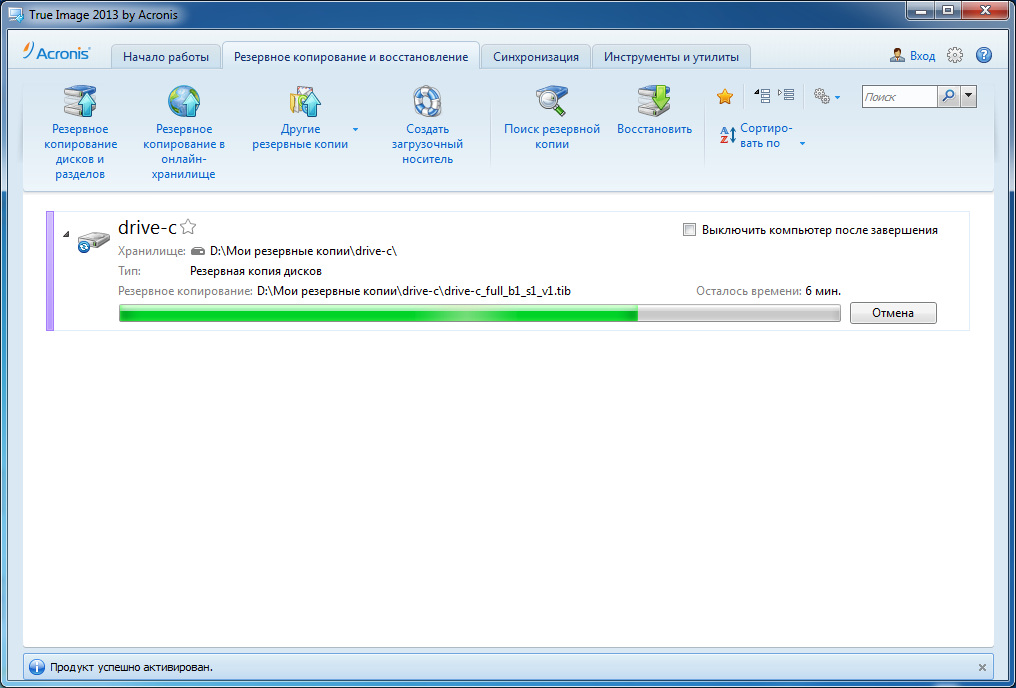
\includegraphics[height = 8\baselineskip]{./assets/y03s01-pcdiag-lab-04-p01.png}
					\caption{}
					\label{subfig:01-01}
				\end{subfigure}%
				\begin{subfigure}{0.5\columnwidth}
					\centering
					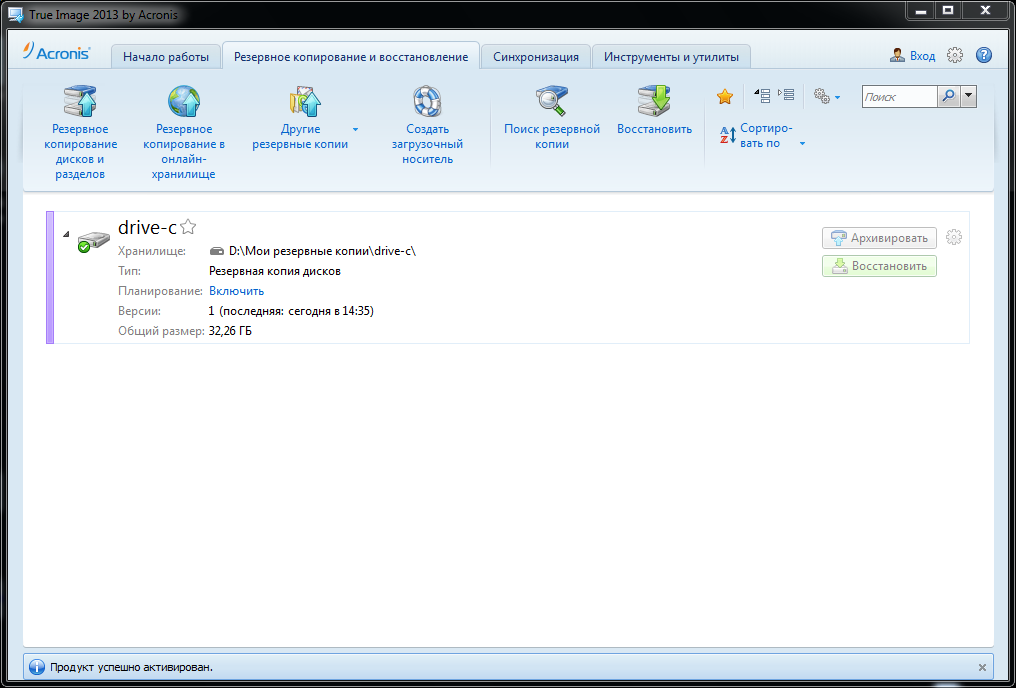
\includegraphics[height = 8\baselineskip]{./assets/y03s01-pcdiag-lab-04-p02.png}
					\caption{}
					\label{subfig:01-02}
				\end{subfigure}%
				\caption{Результат створення резервної копії програмою~\textenglish{Acronis True Image 2013}}
				\label{fig:01-acronis-true-image-res}
			\end{figure}

		\subsection{Створення резервної копії за~допомогою завантажувального диска~\textenglish{Acronis True Image 2014}}
		\label{ssec:acronis-true-image-2014-backup}
			Налаштовуємо комп'ютер на завантаження з диску~\textenglish{Acronis True Image 2014} та перезавантажуємо його. У з'явившомуся меню обираємо пункт~\textenglish{«Acronis True Image 2014»} та натискаємо на нього. Виконалось завантаження необхідної підсистеми. Для створення резервної копії системи обираємо підпункт «Резервне копіювання» \Mytextrightarrow «Диски», позначаємо системний диск \textenglish{C:}, та натискаємо на кнопку «Далі». У з'явившомуся вікні «Цільовий архів резервних копій» обираємо пункт «Створити новий архів резервних копій», обираємо шлях для збереження копії та натискаємо кнопку «Далі». Перевіряємо деталі резервного копіювання у з'явившомуся вікні та натискаємо кнопку «Приступити»~— розпочнеться процес резервного копіювання~(рис.~\ref{subfig:02-01-acronis-true-image-disk-backup-inprocess}). Після закінчення процесу програма звітує про успішне виконання~(рис.~\ref{subfig:02-01-acronis-true-image-disk-backup-res}).

			\begin{figure}[!htbp]
				\centering
				\begin{subfigure}{0.5\columnwidth}
					\centering
					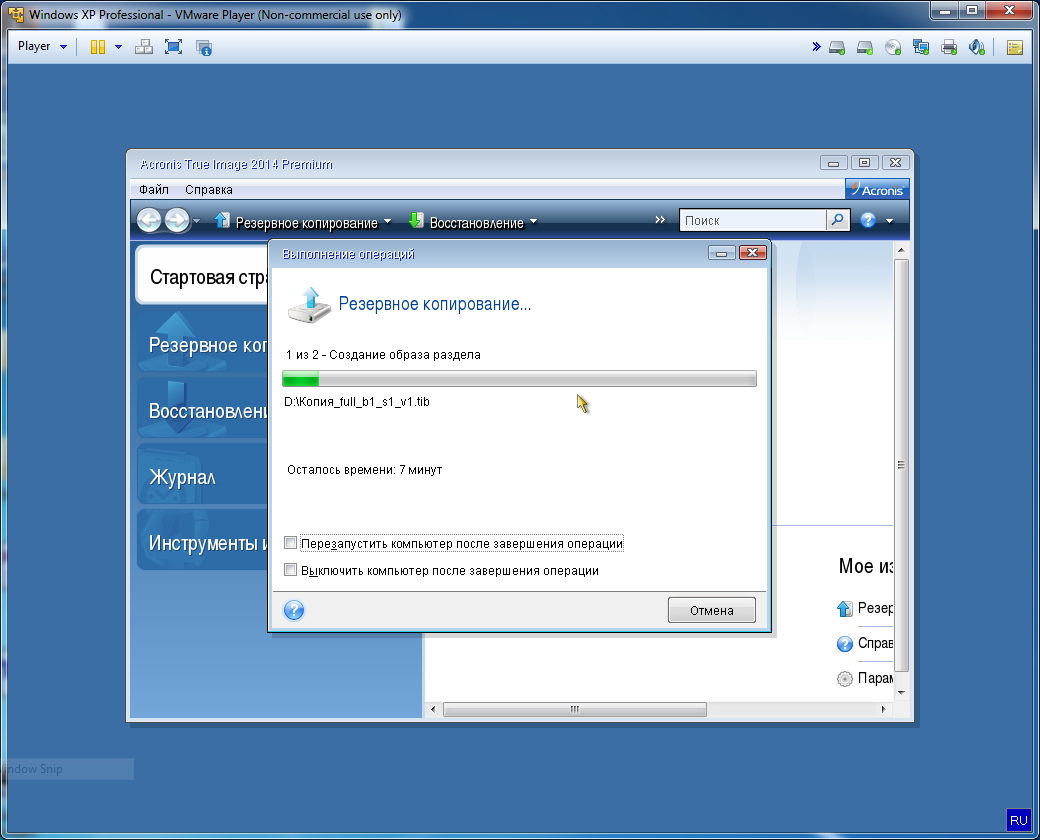
\includegraphics[height = 8\baselineskip]{./assets/y03s01-pcdiag-lab-04-p03.png}
					\caption{}
					\label{subfig:02-01-acronis-true-image-disk-backup-inprocess}
				\end{subfigure}%
				\begin{subfigure}{0.5\columnwidth}
					\centering
					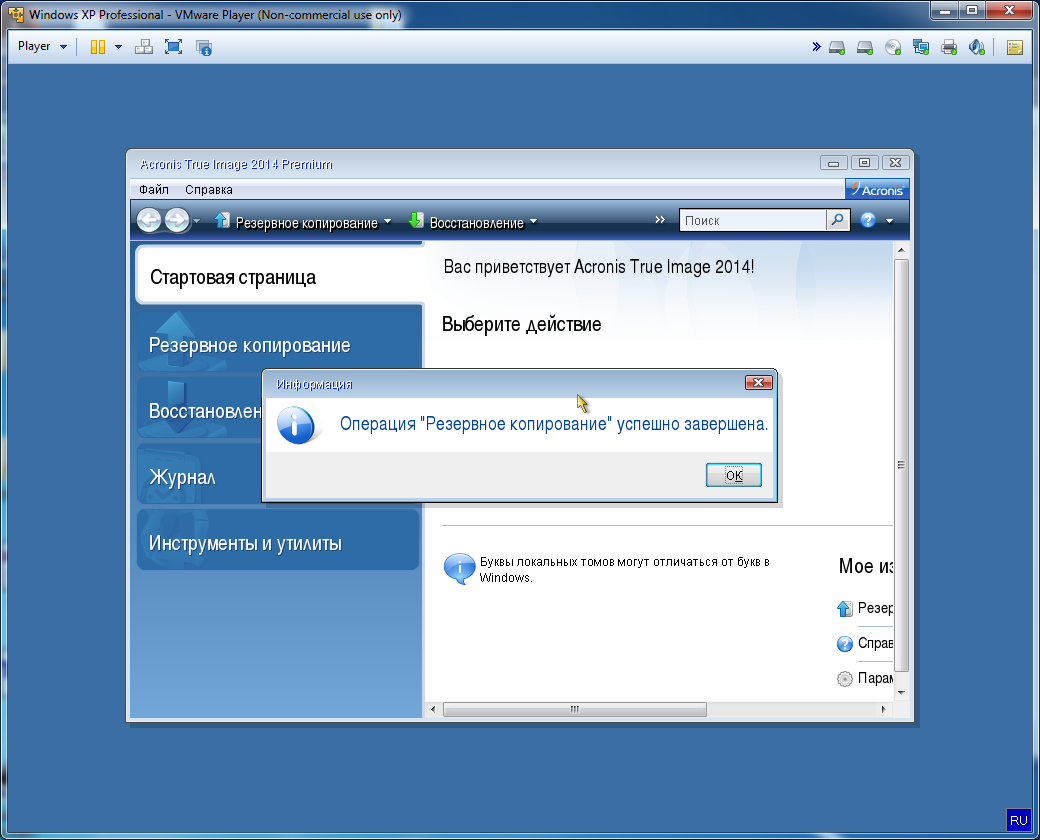
\includegraphics[height = 8\baselineskip]{./assets/y03s01-pcdiag-lab-04-p04.png}
					\caption{}
					\label{subfig:02-01-acronis-true-image-disk-backup-res}
				\end{subfigure}%
				\caption{Результат створення резервної копії завантажувальним диском~\textenglish{Acronis True Image 2014}}
				\label{fig:02-acronis-true-image-disk-backup-res}
			\end{figure}

		\subsection{Відновлення резервної копії за~допомогою завантажувального диска~\textenglish{Acronis True Image 2014}}
			Повертаємось до стартової сторінки~\textenglish{Acronis True Image 2014} та обираємо підпункт «Відновлення»~\Mytextrightarrow «Диски». Обираємо резервну копію, створену у підпункті~\ref{ssec:acronis-true-image-2014-backup} та натискаємо «Далі». Встановлюємо режим «Відновити диски чи розділи», натискаємо «Далі». У вікні, що з'явилось, обираємо елементи для встановлення та натискаємо «Далі». Після перевірки обраних налаштувань запускаємо процес відновлення~(рис.~\ref{fig:03-acronis-true-image-disk-restore}).

			\begin{figure}[!htbp]
				\centering
				\begin{subfigure}{0.5\columnwidth}
					\centering
					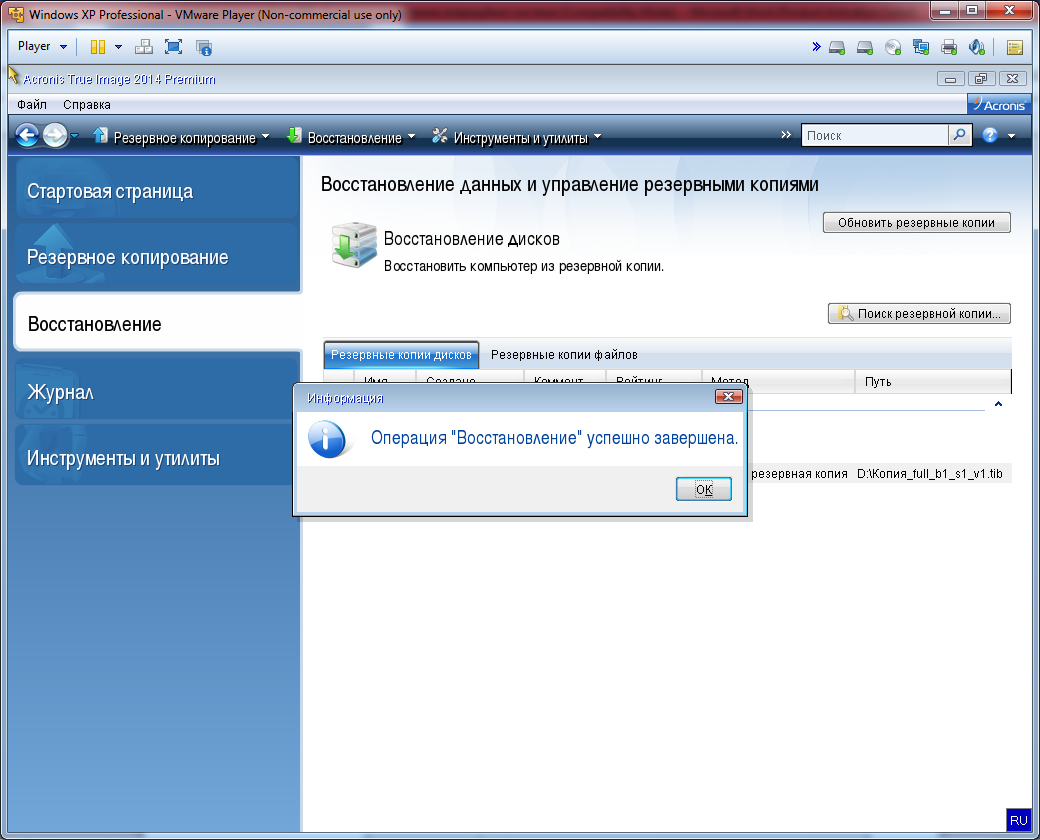
\includegraphics[height = 8\baselineskip]{./assets/y03s01-pcdiag-lab-04-p05.png}
					\caption{}
					\label{subfig:03-01-acronis-true-image-disk-restore-inprocess}
				\end{subfigure}%
				\begin{subfigure}{0.5\columnwidth}
					\centering
					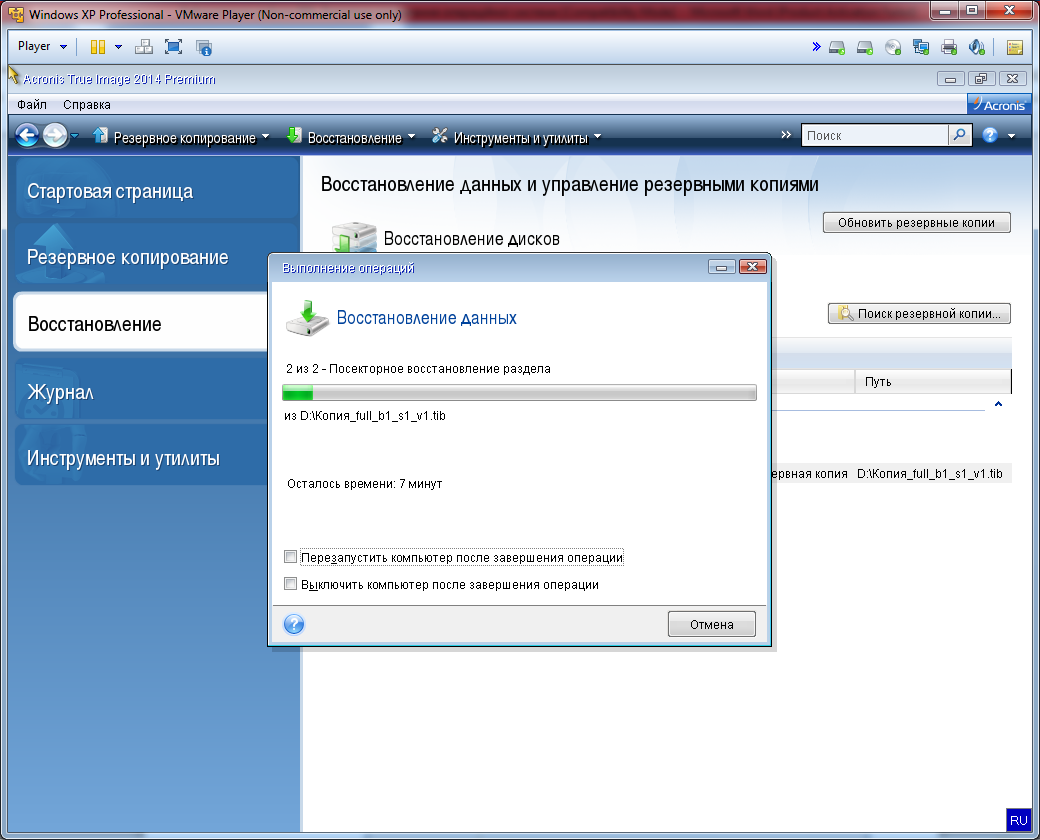
\includegraphics[height = 8\baselineskip]{./assets/y03s01-pcdiag-lab-04-p06.png}
					\caption{}
					\label{subfig:02-01-acronis-true-image-disk-restore-res}
				\end{subfigure}%
				\caption{Результат відновлення резервної копії завантажувальним диском~\textenglish{Acronis True Image 2014}}
				\label{fig:03-acronis-true-image-disk-restore}
			\end{figure}

		\subsection{Створення точки відновлення~\textenglish{Windows}}
			Переконуємось у тому, що на тестовому комп'ютері увімкнено відновлення системи. Для цього переходимо у меню~«Відновлення системи», натиснувши правою клавішею мишки на ярлику «Мій комп'ютер» та обравши відповідну вкладку. Бачимо, що для всіх підключених дисків функція Відновлення системи ввімкнена~(рис.~\ref{fig:04-windows-sysrestore-disk-status}).

			\begin{figure}[!htbp]
				\centering
				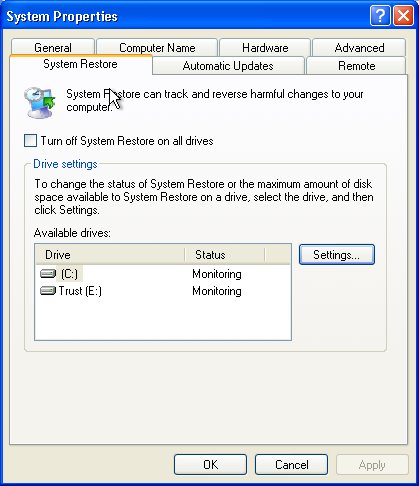
\includegraphics[height = 8\baselineskip]{./assets/y03s01-pcdiag-lab-04-p07.png}
				\caption{Статус Відновлення системи~\textenglish{Windows}}
				\label{fig:04-windows-sysrestore-disk-status}
			\end{figure}

			Створюємо точку відновлення, для чого переходимо в~меню~«Пуск»~\Mytextrightarrow «Всі програми»~\Mytextrightarrow «Стандартні»~\Mytextrightarrow «Службові»~\Mytextrightarrow «Відновлення системи», обираємо пункт «Створити точку відновлення» та додаємо її опис~(рис.~\ref{fig:05-windows-sysrestore-creation}).

			\begin{figure}[!htbp]
				\centering
				\begin{subfigure}{0.5\columnwidth}
					\centering
					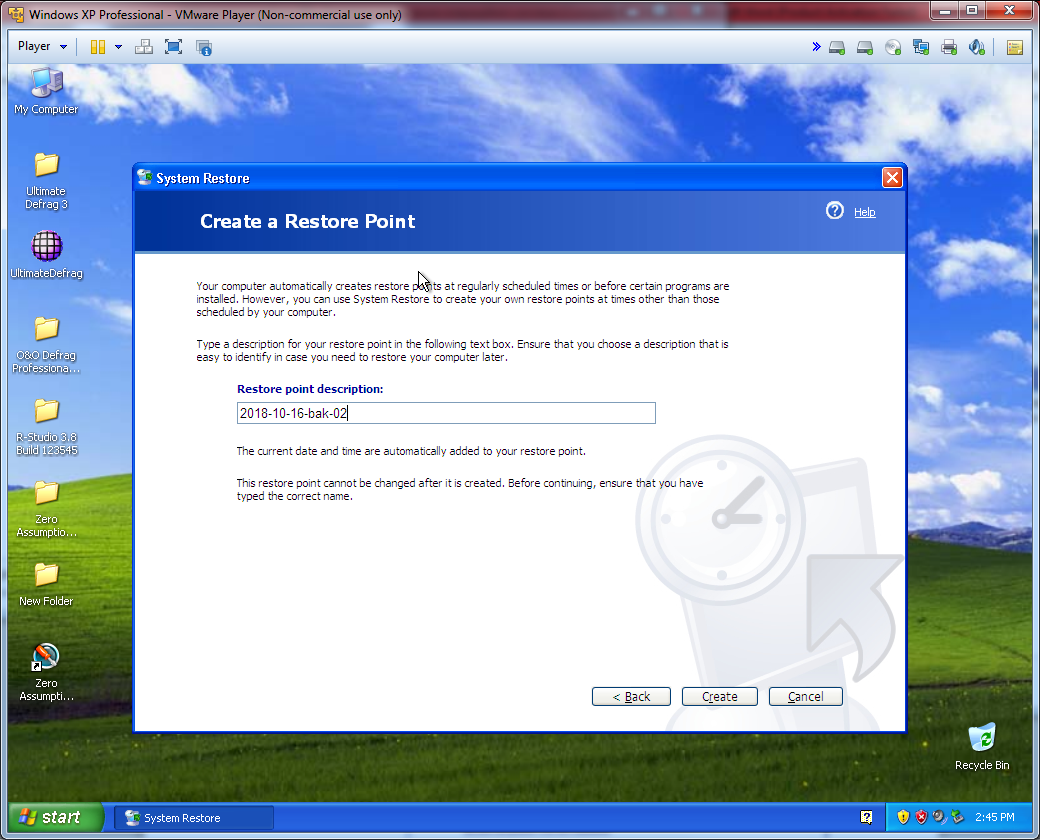
\includegraphics[height = 8\baselineskip]{./assets/y03s01-pcdiag-lab-04-p08.png}
					\caption{}
					\label{subfig:05-01-windows-sysrestore-creation-start}
				\end{subfigure}%
				\begin{subfigure}{0.5\columnwidth}
					\centering
					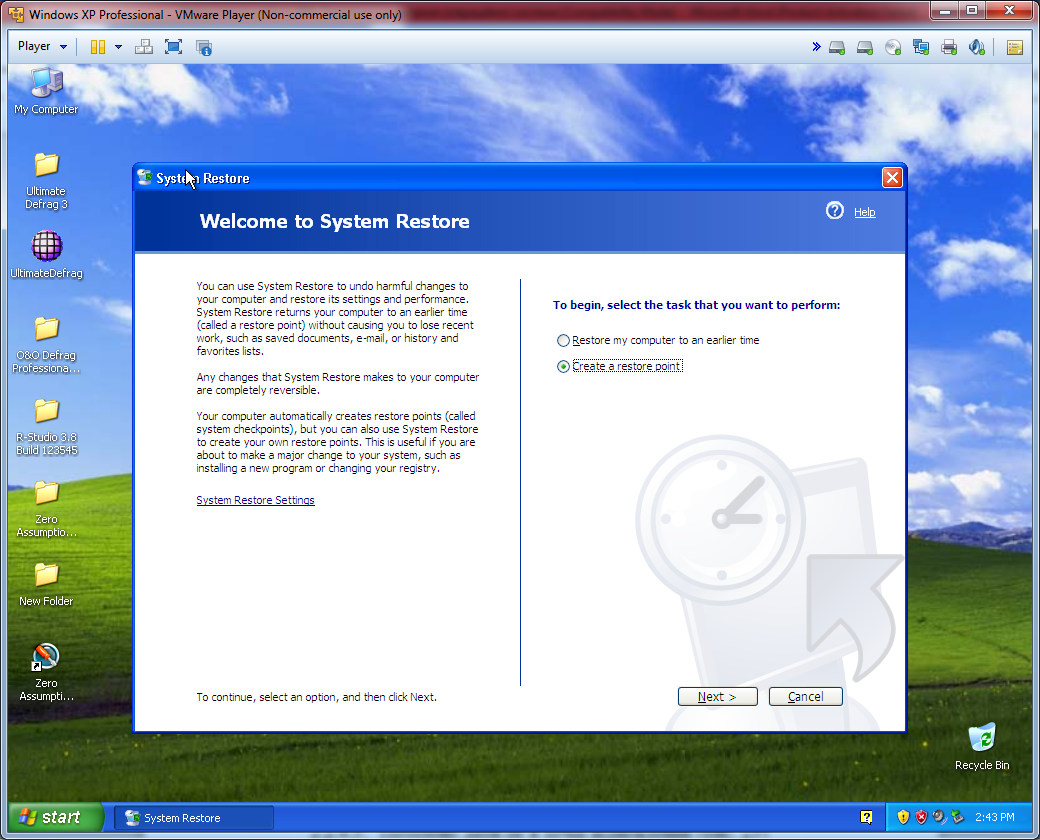
\includegraphics[height = 8\baselineskip]{./assets/y03s01-pcdiag-lab-04-p09.png}
					\caption{}
					\label{subfig:05-01-windows-sysrestore-creation-finish}
				\end{subfigure}%
				\caption{Створення точки відновлення~\textenglish{Windows}}
				\label{fig:05-windows-sysrestore-creation}
			\end{figure}

			Після створення точки, запускаємо відновлення з неї, для чого переходимо в~меню~«Пуск»~\Mytextrightarrow «Всі програми»~\Mytextrightarrow «Стандартні»~\Mytextrightarrow «Службові»~\Mytextrightarrow «Відновлення системи», обираємо пункт «Відновлення попереднього стану комп'ютера», обираємо необхідну дату і точку відновлення, перевіряємо обрані параметри та запускаємо процес~(рис.~\ref{fig:06-windows-sysrestore-selection}).

			\begin{figure}[!htbp]
				\centering
				\begin{subfigure}{0.5\columnwidth}
					\centering
					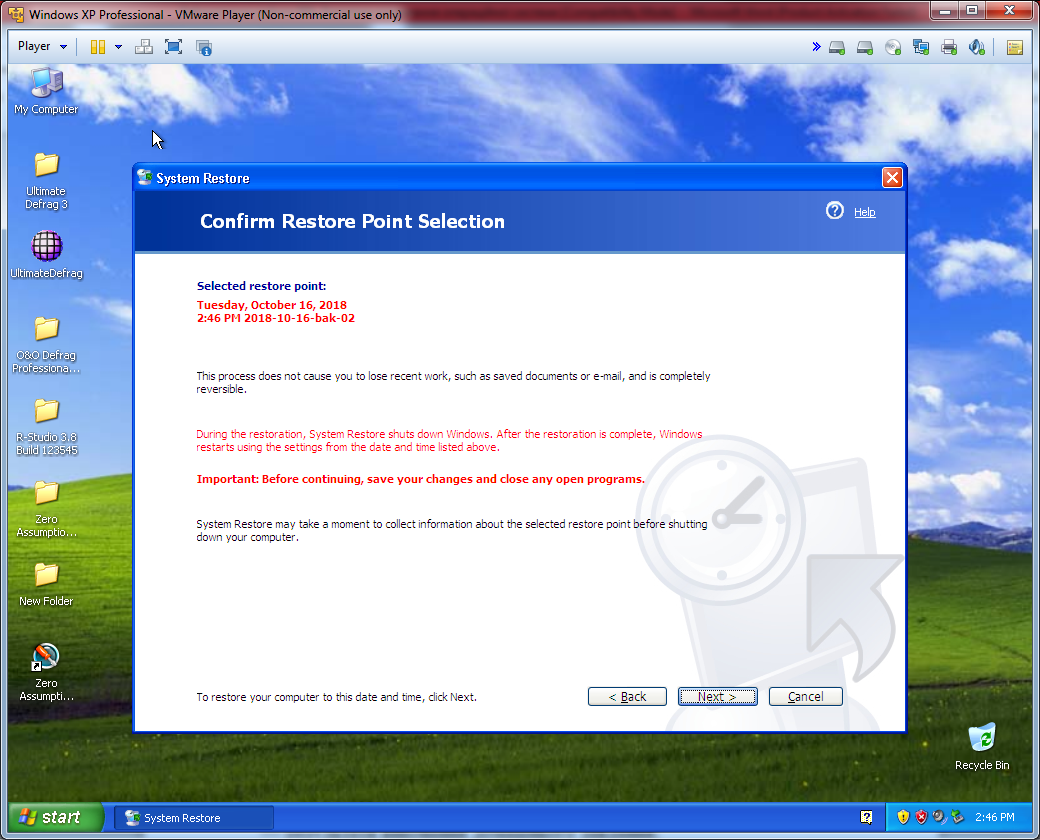
\includegraphics[height = 8\baselineskip]{./assets/y03s01-pcdiag-lab-04-p10.png}
					\caption{}
					\label{subfig:06-01-windows-sysrestore-selection-start}
				\end{subfigure}%
				\begin{subfigure}{0.5\columnwidth}
					\centering
					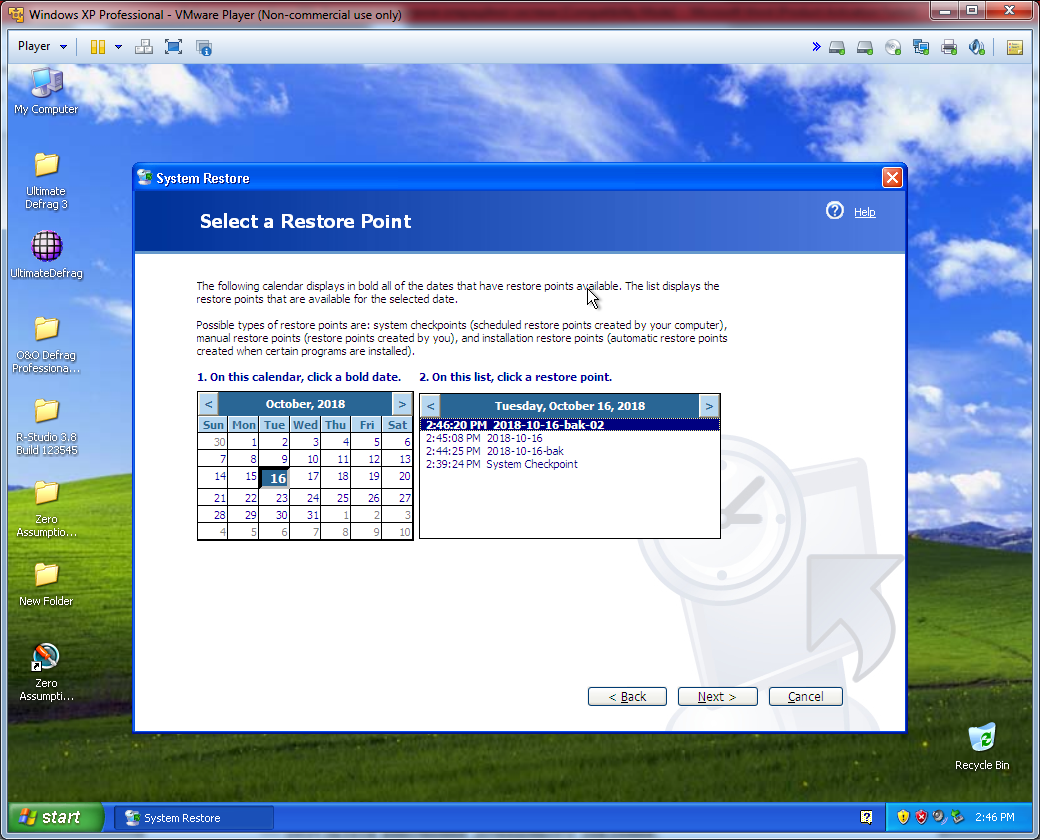
\includegraphics[height = 8\baselineskip]{./assets/y03s01-pcdiag-lab-04-p11.png}
					\caption{}
					\label{subfig:06-01-windows-sysrestore-selection-finish}
				\end{subfigure}
				%
				\begin{subfigure}{0.5\columnwidth}
					\centering
					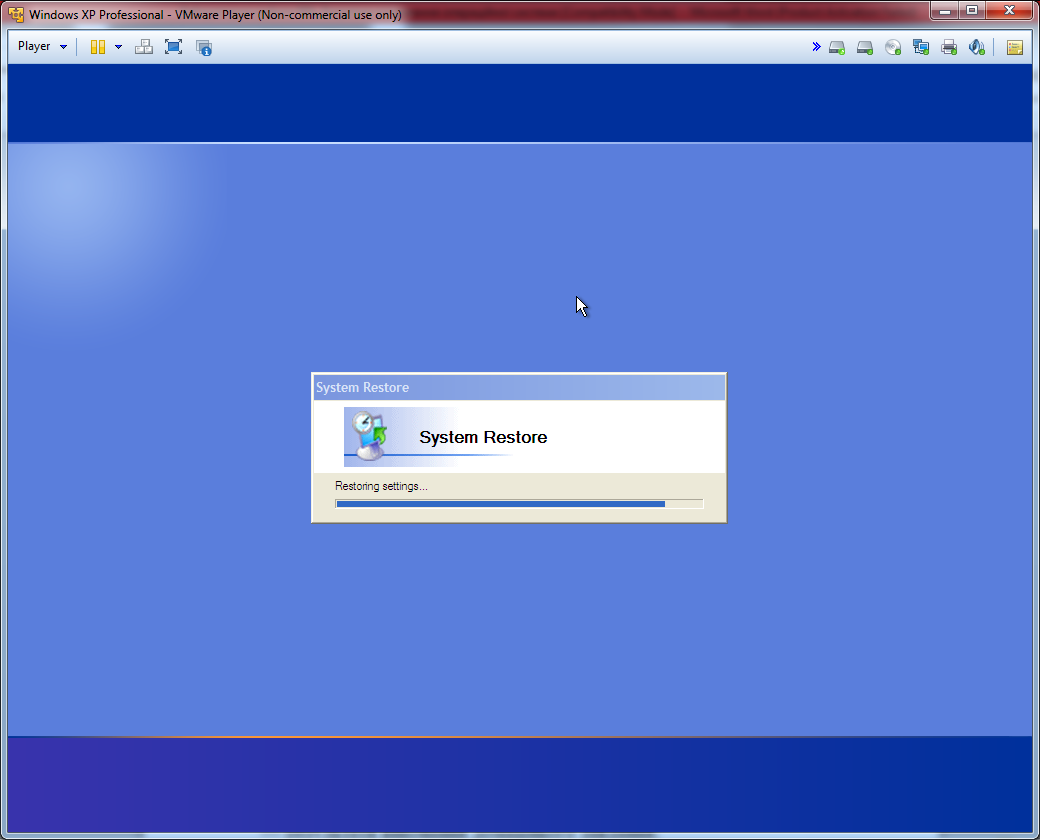
\includegraphics[height = 8\baselineskip]{./assets/y03s01-pcdiag-lab-04-p12.png}
					\caption{}
					\label{subfig:06-03-windows-sysrestore-restoration-start}
				\end{subfigure}%
				\begin{subfigure}{0.5\columnwidth}
					\centering
					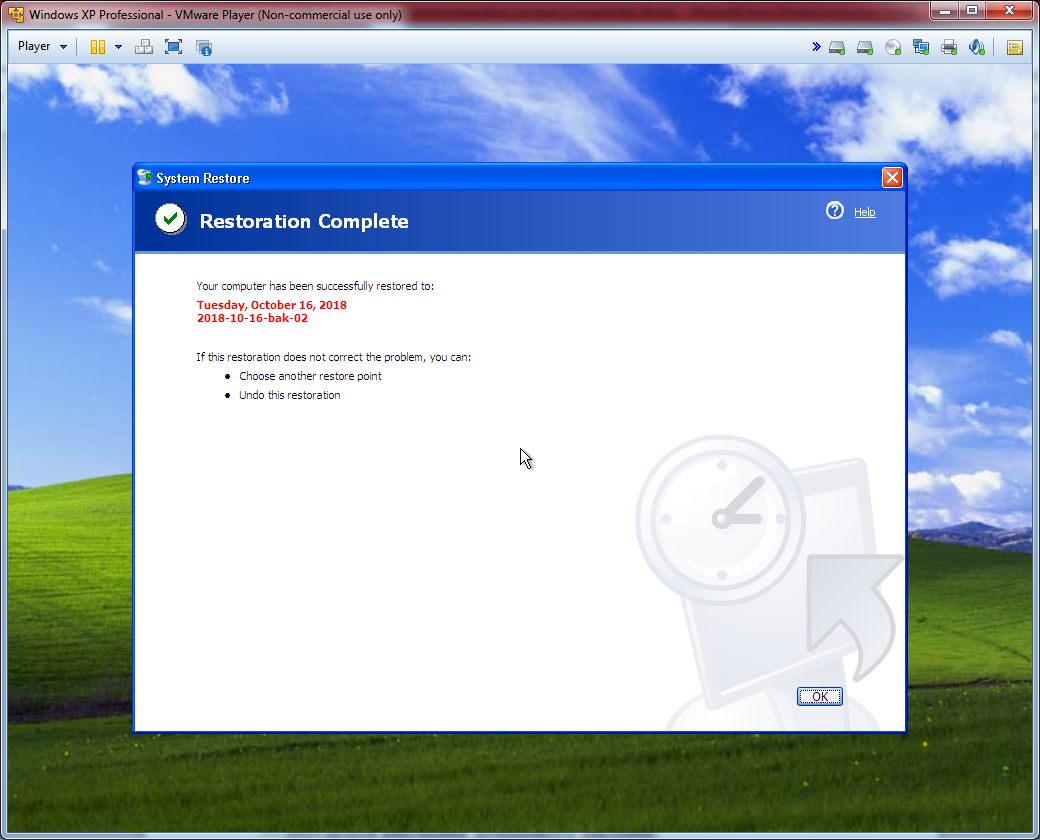
\includegraphics[height = 8\baselineskip]{./assets/y03s01-pcdiag-lab-04-p13.png}
					\caption{}
					\label{subfig:06-04-windows-sysrestore-restoration-finish}
				\end{subfigure}%
				\caption{Відновлення зі~створеної точки відновлення~\textenglish{Windows}}
				\label{fig:06-windows-sysrestore-selection}
			\end{figure}

		\section{Висновки}
			Під час виконання даної лабораторної роботи ми ознайомились з процесом резервного копіювання та відновлення операційної системи на прикладі програм~\textenglish{Acronis True Image Home 2013}, завантажувального диску~\textenglish{Acronis True Image Home 2014} та стандартного засобу операційної системи~\textenglish{Windows} «Відновлення системи».

\end{document}
